\documentclass[a4paper, 12pt]{article}

\usepackage[utf8]{inputenc}
\usepackage[T1]{fontenc}
\usepackage[french]{babel}
\usepackage[top=2cm, bottom=2cm, left=1.5cm, right=1.5cm,headheight=16pt]{geometry}
\usepackage{lmodern}

\addto\captionsfrench{%
    \renewcommand{\tablename}{\textsc{Tableau}}%
}

\usepackage{cover-page}
\title{Finite State Transducers Just-In-Time Compiling}
\subtitle{Do you hear the bytecode ?}
\author{Émilien Boulben\\Victor Delepine\\Corentin Peuvrel}
\location{Paris}
\date{\today}
\blurb
{
    Institut Supérieur d'Électronique de Paris\\
    \textbf{Projet de Fin d'Études}\\
    ~\\
    Reponsable: M. Hugueney
}

\usepackage{fancy-perso}
\usepackage{lastpage}
\headerleft{Finite State Transducer Just-In-Time Compiling}
\headerright{Institut Superieur d'Électronique de Paris}
\footerleft{É.Boulben, V.Delepine, C.Peuvrel}
\footerright{\hyperlink{Contents}{Table des matières}}

\usepackage{parskip}
\setlength{\parindent}{18pt}

\usepackage{listings}
\usepackage{upquote}
\usepackage{graphicx}
\usepackage{listings}
\usepackage{xcolor}

\makeatletter
\newcommand{\lstdefinestylecustom}[3] {%
    \ifnum\pdfstrcmp{#3}{x86masm}=0
    \lstdefinestyle{#1}{
        numbers=left,
        stepnumber=1,
        numberstyle=\scriptsize,
        belowcaptionskip=1\baselineskip,
        captionpos=b,
        breaklines=true,
        frame=L,
        xleftmargin=\parindent,
        language=[#3]#2,
        showstringspaces=false,
        basicstyle=\footnotesize\ttfamily,
        keywordstyle=\bfseries\color{green!40!black},
        commentstyle=\itshape\color{purple!40!black},
        identifierstyle=\color{blue},
        stringstyle=\color{orange},
        comment=[l]\#,
    }
    \else
    \lstdefinestyle{#1}{
        numbers=left,
        stepnumber=1,
        numberstyle=\scriptsize,
        belowcaptionskip=1\baselineskip,
        captionpos=b,
        breaklines=true,
        frame=L,
        xleftmargin=\parindent,
        language=#2,
        showstringspaces=false,
        basicstyle=\footnotesize\ttfamily,
        keywordstyle=\bfseries\color{green!40!black},
        commentstyle=\itshape\color{purple!40!black},
        identifierstyle=\color{blue},
        stringstyle=\color{orange},
    }
    \fi
}
\makeatother

\lstdefinestylecustom{custombash}{bash}{}
\lstdefinestylecustom{customc}{C}{}
\lstdefinestylecustom{customasm}{Assembler}{x86masm}

\usepackage[pdftex,breaklinks,linktocpage,unicode]{hyperref}
\hypersetup{
    unicode=false,          % non-Latin characters in Acrobat’s bookmarks
    pdftoolbar=true,        % show Acrobat’s toolbar?
    pdfmenubar=true,        % show Acrobat’s menu?
    pdffitwindow=false,     % window fit to page when opened
    pdfstartview={FitH},    % fits the width of the page to the window
    pdftitle={Finite State Transducer Just-In-Time Compiling},    % title
    pdfauthor={Émilien Boulben, Victor Delépine, Corentin Peuvrel},     % author
    pdfsubject={FST, bytecode, optimisation},   % subject of the document
    pdfcreator={Émilien Boulben},   % creator of the document
    pdfproducer={Émilien Boulben}, % producer of the document
    pdfkeywords={FST, assembler, bytecode, just, time, java}, % list of keywords
    pdfnewwindow=true,      % links in new window
    colorlinks=true,       % false: boxed links; true: colored links
    linkcolor=black,          % color of internal links (change box
    % color with linkbordercolor)
    linktoc=all,
    citecolor=green,        % color of links to bibliography
    filecolor=magenta,      % color of file links
    urlcolor=cyan           % color of external links
}


\usepackage{amsmath}

\begin{document}

\maketitle

\newpage
\clearpage
\pagenumbering{Roman}
\setcounter{page}{1}
\footercenter{\textbf{\thepage}}
\fancyperso{HL}{HR}{FL}{FC}{}

\hypertarget{Contents}{}
\tableofcontents
\newpage
\lstlistoflistings
\newpage
\listoftables
\newpage
\listoffigures

\newpage
\clearpage
\pagenumbering{arabic}
\setcounter{page}{1}
\footercenter{\textbf{Page \thepage/\pageref{LastPage}}}
\fancyperso{HL}{HR}{FL}{FC}{FR}

\section*{Introduction}
\addcontentsline{toc}{section}{\protect\numberline{}Introduction}

Les FST -- Finite State Transducers ou en français Transducteur fini -- sont des automates
finis particuliers puique possédant une sortie. Ils sont enormément utilisés par les
moteurs de recherche puisqu'ils permettent d'associer à un mot une valeur numérique
unique. C'est l'indexation.


Nous savons donc déjà transformer le texte en valeur exploitable ensuite
(par comparaison avec un disctionnaire par exemple).
Mais de part les quantités non négligeable de texte à analyser, et ce le plus rapidement
possible, il est essentiel de continuer les recherches afin de réussir à optimiser
cette transformation.


Seulement en ingénérie l'optimisation n'est pas tout, il faut aussi pouvoir simplement déployer les
solutions sur différents serveurs : une solution trop complexe même performante sera très
coûteuse à long termes et donc probablement pas choisie.
C'est alors qu'intervient ce projet.


Il s'agit de faire une étude sur la faisabilité et la pertinence d'une nouvelle manière
d'indexer le texte en java, L'objectif n'est pas de faire mieux que la référence qu'est Lucène,
mais de déterminer s'il est possible de faire mieux en utilisant cette méthode.\newline


Nous allons avec ce projet chercher à déterminer si un interpréteur de FST reposant sur la
compilation à la volée est viable en java.

\newpage
\section{Analyse préalable}

\subsection{Le projet en détail}

Pour pallier à des problèmes de performance et de distribution de la solution lors de
l'indexation d'un texte en suivant une FST il est important de penser à de nouvelles
solutions qui pourront éventuellement challenger la librairie de référence sur ce sujet :
Lucène. L'objectif n'est pas d'y parvenir, mais de déterminer si cela est possible avec
une solution qui a été imaginée par M. Hugueney et M. Marty.


Dans Lucène lors de la création d'une FST une structure de données est stockée en ram et
le texte la parcourt pour connaître le résultat. Afin de gagner en performance en termes
de temps d'exécution lors de cette étape, ne serait-il pas mieux de pouvoir avoir un code
simple mais conséquent en taille qui soit parfaitement adapté à la FST désirée ? Finalement,
plutôt que créer une structure générique, générer un code dédié à la FST en étude et l'optimiser
au mieux en bafouant tous les principes de développement afin de gagner en temps d'exécution.
La lisibilité est sacrifiée mais ce n'est pas très important compte tenu que ce code n'a pas
destination à être lu, seulement compilé puis parcouru.\newline


L'objectif du projet est de réussir à créer un programme Java qui génèrerait le code correspondant
à une FST donnée pour pouvoir parser du texte efficacement, d'abord en Java puis en bytecode.
Ensuite, faire une étude des performances et si possible les comparer avec les outils déjà existant.
Il est très important de documenter les difficultés rencontrées puisque l'objectif reste de
pouvoir se prononcer sur la faisabilité ou l'utilité d'un tel produit.

\subsection{Premières études}

Il nous a été très compliqué de comprendre ce qu'était une FST. Nous avons beaucoup investi de
temps à combler ce manque avec des résultats très mitigés. Il était très difficile avec toute la
documentation disponible de savoir par quoi commencer, surtout que souvent pour comprendre
certains concepts il nous fallut assimiler ce que les explications considéraient acquit.

Cette incompréhension du sujet fût à l'origine de bien des découragements, et il n'a pas toujours
été facile de nous remotiver les uns et les autres. Finalement c'est la pratique qui nous a apporté
le plus de réponse.\newline

Une FST qui permette l'indexation de texte, qu'est-ce ? Une simple structure de donnée. Un tableau
(voir \autoref{tab:fst1} et \autoref{tab:fst2}) ou un graphe (voir \autoref{fig:fst-dico1} et \autoref{fig:fst-dico2} peut la représenter.
Elle est construite par un algorithme à partir d'un dictionnaire qui associe à des mots des valeurs.
Enfin cela permet de parser du texte lettre à lettre (voir mots à mots) rapidement et en parallèle.


Une fois cette base essentielle partiellement comprise nous avons pris le courage de nous lancer
dans le code.

\subsection{Commencer quelque part}

Commencer à coder paraît simple et pourtant nous y avons rencontré de trop nombreuses difficultés.
Nous nous sommes heurtés à des nombreuses reprises à notre méconnaissances des FST, et n'arrivions
pas à dégager un cas simple sur lequel travailler et monter en compétence.

Nous avons aussi perdu du temps à partir sur du code inutile à ce moment du développement :
algorithmes de création d'une FST, tests en bytecode... Alors que ce n'était pas la priorité
à ce moment.\newline


C'est après une pause dans le projet que nous avons pu le reprendre d'un regard nouveau et
l'aborder avec un outil que nous maitrisons mieux pour générer du text : bash. Par un découragement
général nous avons presqu'involontairement trouvé ce dont nous avions besoin pour nous lancer
avec efficacité dans le projet : un appui solide mais rapide à construire.

\newpage
\section{Les premiers essais}

\subsection{Générer du C en bash}

L'objectif ici n'était pas de réussir à faire quelque chose de fonctionnel, mais de comprendre
ce qu'il nous fallait faire. Pour ce faire nous avons finalement décidé de le faire avec les
langages que nous maitrisions le plus et que nous jugions les plus adaptés pour la situation : le
bash et le C.

\subsubsection{Le jeu de données}

Nous avons créé manuellement des FST très basique, reliées à un dictionnaire, afin de disposer
d'un jeu de test. Ils se trouvent en \autoref{sec:annexe:shell}.

Nous avons légèrement adapter le format défini par AT\&T opur décrire des FST dans un fichier texte.
CE jeu de données servira pendant tout le projet en étant réadapté en Java par la suite.

\subsubsection{Fonctionnement}

Dans ce premier test nous prenons en entrée du script le fichier texte décrivant la FST,
puis générons un code C qui permette de parcourir cette FST.
Dans ce nouveau code point d'alorithme complexe : simplicité et naïvité sont ici ce que nous cherchons.
Nous espérons alors que la pratique nous permettra
de mieux comprendre le sujet.
De plus nous faisons confiance à gcc pour optimiser le code à la compilation.


La première étape pour construire ce script est bien sûr de prévoir la forme qu'aura le code C généré :
nous avons donc concentré nos premiers efforts à la généation d'une fonction contenant de multiples labels
correspondant chacun à un état (ou n\oe ud) et un switch qui, suivant la lettre courrante
se déplace à la lettre suivante grâce à un goto qui pointe sur le label du state/node suivant.
Nous returnons un code d'erreur si le token d'entrée n'est pas compatible avec la FST (le mot n'est pas
pris en compte par celle-ci et n'a pas de code associé).



Cette fonction prend comme seul paramètre d'entrée une chaine (tableau de char) --
qui sera le token d'entrée dont on veut connaitre la valeur -- et retourne le poids cumulé de
tous les arcs traversés, ou -1 en cas d'erreur.
Il faut remarquer qu'avec cette méthode on ne peut pas supporter de poids négatifs,
au risque d'avoir une collision entre le code d'erreur et un poids cumulé effectivement négatif.
Pour gérer ce cas, le plus simple serait d'utiliser errno.

Le code a été un peu moins simple que prévu pour pouvoir générer du C valide, en effet, il y a un
certain nombre de cas particuliers à prendre en compte afin de gérer correctement les erreurs ou
de multiples états de fins.



Au final, un état générera un code semblable à celui présent dans le \autoref{lst:node:example}
(pour un état appellé "7", qui possède
un arc pour le caractère 'X' avec un poids de 6 et qui va au node "21", et un arc pour
le caractère 'Y' avec un poids nulle et allant au node "42").
\begin{figure}
    \lstinputlisting[style=customc, caption=Un example de code généré pour un état,label=lst:node:example]{code/node1}
\end{figure}

On remarque la présence d'un compteur "pos" incrémenté de manière inconditionnel, vu que l'on se
déplace toujours un caractère par un caractère.

Pour pouvoir facilement lancer le programme généré, nous avons rajouté une fonction main qui appelle
juste notre fonction compute\_fst sur le premier argument de la command line,
rendant ainsi le programme autonome.

Il nous suffit donc, pour générer quelque chose d'utilisable de faire ceci :

\begin{align*}
    ./gen.sh\ file.fst\ |\ gcc\ -x\ c\ -o\ fst\ -
\end{align*}

Puis :

\begin{align*}
./fst\ LE\_TOKEN
\end{align*}

Les options sur gcc (on peut aussi rajouter un -O3 pour optimiser au maximum la compilation)
servant seulement de prendre l'entrée standard comme "fichier" source, puisque gen.sh affiche
le code généré sur la sortie standard.\newline


Les différents codes se situent en \autoref{sec:annexe:shell:c}, et plus précisément :
\begin{itemize}
    \item code bash : \autoref{lst:bashgen}
    \item Premier example de code C obtenu : \autoref{lst:cfst1}
    \item Second example de code C obtenu : \autoref{lst:cfst2}
\end{itemize}

\subsubsection{Les avantages}

Si le résultat n'avait que peu d'importance ici, ce début à une importance capitale dans ce projet
puisque c'est ce petit code qui nous a permis de mieux comprendre ce qui était attendu de nous,
comment le faire, et comment utiliser une FST.

\subsection{Générer de l'asmX86 en bash}

Sachant qu'on devrait sûrement au final généré du bytecode, nous avons décidé que, quitte à avoir du C,
autant aller jusqu'à générer directement de l'assembleur.
Pas spécialement pour être plus performant que le C (en effet, l'assembleur  généré par gcc
sera toujours plus efficace que celui que l'on peut faire à la main), mais pour avoir des idées
des problèmes que nous rencontrerons en bytecode.

Quand nous parlons d'assembleur, nous entendons "assembleur x86\_64" bien sûr,
soit l'assembleur qui est généré par gcc sur nos machines.


En donnant l'option "-S" à gcc, on obtient non pas un binaire éxécutable
mais un fichier ".s" qui contient le code assembleur généré (avant l'assemblage effectif en binaire).
En le générant pour nos sources C, nous avons pu faire du rétro-engineering dessus
et comprendre la marche à suivre pour notre deuxième script.

La première partie, pour adapter toutes les parties générées de manière statique, a été relativement aisée.
Par exemple, la déclaration de la fonction main, bien que plus longue et moins lisible qu'en C pouvait
être plus ou moins copié/collé par rapport à ce que générait gcc, et même si quelques lignes restaient
un peu mystérieuses au moment de la mise en place de "l'environnement" de la fonction, ce n'était
absolument pas bloquant.

À l'opposé, lorsqu'il a fallu adapter les parties générées dynamiquement, ce fut beaucoup moins simple.
Nous avons du, l'espace d'un instant, changer notre façon de programmer. En effet, l'assembleur
est tellement bas niveau que l'on ne dispose pas de toutes les "syntactic sugar" dont on a
tant l'habitude, nottamment pour le contrôle de flux. Par exemple, ce n'est pas si simple que
ce à quoi nous pourrions nous attendre de faire un "if (...) single\_instruction ;".
Il faut gérer deux sauts, les labels associés, potentiellement préparer un ou deux registres, etc...


Ce fût très amusant à faire, et moins complexe qu'imaginé grâce à l'exhaustivité de la documentation.
Néanmoins le temps passé dessus ne s'est révélé être aussi utile qu'escompté car nous le découvrirons
plus tard les problèmes rencontrés pour le bytecode sont d'un ordre totalement différents.\newline


Les différents codes se situent en annexe,annexe \autoref{sec:annexe:shell:asm}, et plus précisément :
\begin{itemize}
    \item code bash : \autoref{lst:bashgenasm}
    \item Premier example de code C obtenu : \autoref{lst:asmfst1}
    \item Second example de code C obtenu : \autoref{lst:asmfst2}
\end{itemize}

\newpage
\subsection{Adopter le travail précédent en Java}

\subsection{Générer une structure de switch imbriqués en Java}

\newpage
\section{Générer une FST}

\newpage
\section{Générer une structure switch en bytecode}

\newpage
\section{Analyse}

\newpage
\section*{Conclusion}
\addcontentsline{toc}{section}{\protect\numberline{}Conclusion}

\newpage
\appendix
\section{Annexe : tests avec un script shell}
\label{sec:annexe:shell}

\subsection{Dictionnaires}

\begin{table}[h]
    \centering
    \begin{tabular}{|l|l|}
        \hline
        Value & Word \\
        \hline
        0 & mop \\
        1 & moth \\
        2 & pop \\
        3 & star \\
        4 & stop \\
        5 & top \\
        \hline
    \end{tabular}
    \caption{Dictionnaire à utiliser avec la FST dans le \autoref{tab:fst1}}
    \label{tab:dico1}
\end{table}

\begin{table}[h]
    \centering
    \begin{tabular}{|l|l|}
        \hline
        Value & Word \\
        \hline
        0 & mop \\
        1 & moth \\
        2 & pop \\
        3 & slop \\
        4 & sloth \\
        5 & stop \\
        6 & top \\
        \hline
    \end{tabular}
    \caption{Dictionnaire à utiliser avec la FST dans le \autoref{tab:fst2}}
    \label{tab:dico2}
\end{table}

\clearpage
\subsection{FST}

\begin{table}[ht]
    \centering
    \begin{tabular}{|l||c|c|c|c|c|c|c|c|c|c|c|c|c|c|c|}
        \hline
        N\oe u & 0 & 0 & 0 & 0 & 1 & 2 & 3 & 2 & 4 & 6 & 7 & 5 & 7 & 8 & \\ \hline
        N\oe u suivant & 1 & 4 & 4 & 6 & 2 & 3 & 9 & 9 & 5 & 7 & 5 & 9 & 8 & 9 & \\ \hline
        N\oe u final &&&&&&&&&&&&&&& 9 \\ \hline
        Caractère & M & P & T & S& O & T & H & P & O & T & O & P & A & R & \\ \hline
        Poids & & 2 & 5 & 3 &&& 1 &&&&1&&&& \\ \hline
    \end{tabular}
    \caption{FST utilisée avec le dictionnaire \autoref{tab:dico1}, voir \autoref{fig:fst-dico1} page \pageref{fig:fst-dico1}}
    \label{tab:fst1}
\end{table}

\begin{figure}[ht]
    \centering
    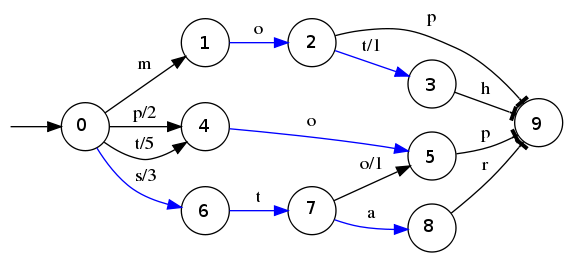
\includegraphics[scale=0.5]{../c_asm/1.png}
    \caption{La FST associée avec le \autoref{tab:fst1} page \pageref{tab:fst1}}
    \label{fig:fst-dico1}
\end{figure}

\begin{table}[ht]
    \centering
    \begin{tabular}{|l||c|c|c|c|c|c|c|c|c|c|c|c|c|c|c|}
        \hline
        N\oe u & 0 & 0 & 0 & 0 & 3 & 3 & 1 & 2 & 4 & 5 & 6 & 5 &\\ \hline
        N\oe u suivant & 1 & 1 & 3 & 4 & 1 & 4 & 2 & 7 & 5 & 6 & 7 & 7 &\\ \hline
        N\oe u final &&&&&&&&&&&&& 7 \\ \hline
        Caractère & P & T & S & M& T & L & O & P & O & T & H & P & \\ \hline
        Poids & 2 & 6 & 3 &  & 2 & & & & & 1 &&& \\ \hline
    \end{tabular}
    \caption{FST utilisée avec le dictionnaire \autoref{tab:dico2}, voir \autoref{fig:fst-dico2} page \pageref{fig:fst-dico2}}
    \label{tab:fst2}
\end{table}

\begin{figure}[!htb]
    \centering
    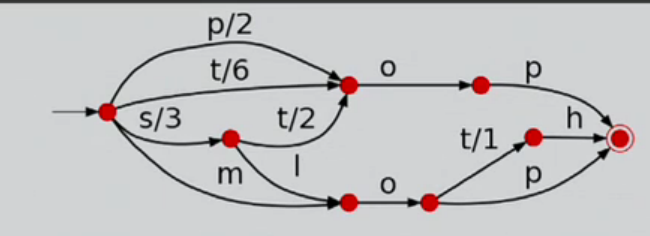
\includegraphics[scale=0.5]{../c_asm/2.png}
    \caption{La FST associée avec le \autoref{tab:fst2} page \pageref{tab:fst2}}
    \label{fig:fst-dico2}
\end{figure}
Les
\clearpage
\subsection{Générer à la volée du code C}
\label{sec:annexe:shell:c}
\subsubsection{Script shell}

\lstinputlisting[style=custombash, caption=Script pour générer un code C à la volée d'une FST,label=lst:bashgen]{../c_asm/gen.sh}

\clearpage
\subsubsection{Code C généré pour la FST définie dans le \autoref{tab:fst1}}

\lstinputlisting[style=customc, caption=Code C généré pour la FST définie dans \autoref{tab:fst1},label=lst:cfst1]{../c_asm/gen_c_fst1.c}

\clearpage
\subsubsection{Code C généré pour la FST définie dans le \autoref{tab:fst2}}

\lstinputlisting[style=customc, caption=Code C généré pour la FST définie dans \autoref{tab:fst2},label=lst:cfst2]{../c_asm/gen_c_fst2.c}


\clearpage
\subsection{Générer à la volée du code assembleur x86}
\label{sec:annexe:shell:asm}
\subsubsection{Script shell}

\lstinputlisting[style=custombash, caption=Script pour générer un code assembleur x86 à la colée d'une FST, label=lst:bashgenasm]{../c_asm/gen_asm.sh}

\clearpage
\subsubsection{Code assembleur x86 généré pour la FST définié dans le \autoref{tab:fst1}}

\lstinputlisting[style=customasm, caption=Code assembleur x86 généré pour la FST définie dans \autoref{tab:fst1}, label=lst:asmfst1]{../c_asm/gen_asm_fst1.asm}

\clearpage
\subsubsection{Code assembleur x86 généré pour la FST définié dans le \autoref{tab:fst2}}

\lstinputlisting[style=customasm, caption=Code assembleur x86 généré pour la FST définie dans \autoref{tab:fst2}, label=lst:asmfst2]{../c_asm/gen_asm_fst2.asm}

\clearpage

\section{Annexe : générer du code java dynamiquement}

\subsection{Dans une seule méthode}

\subsection{Dans différentes méthodes}

\end{document}
